\documentclass[tikz, border=5mm]{standalone}
\usetikzlibrary{fit, positioning}
\begin{document}
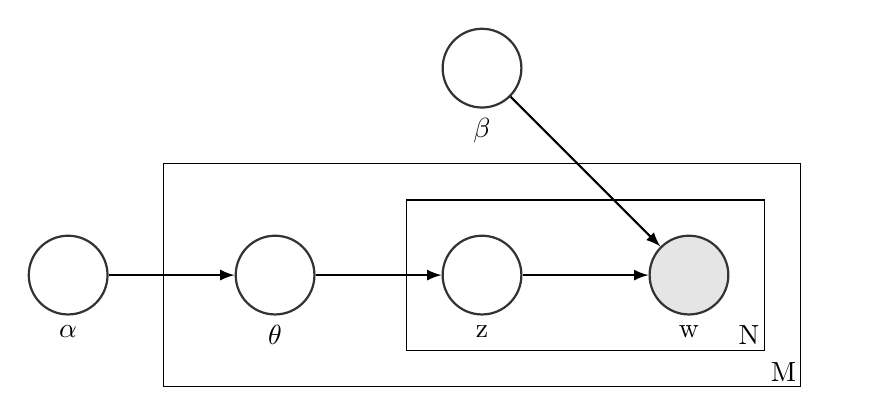
\begin{tikzpicture}

% STYLES
\tikzstyle{main}=[
	circle, minimum size = 10mm, 
	thick, draw =black!80, node distance = 16mm
]
\tikzstyle{connect}=[-latex, thick]
\tikzstyle{box}=[rectangle, draw=black!100]

% NODES
\node [main] (a) [label=below:$\alpha$]             { };
\node [main] (t) [right=of a, label=below:$\theta$] { };
\node [main] (z) [right=of t, label=below:z]        { };
\node [main] (b) [above=of z, label=below:$\beta$]  { };
\node[main, fill = black!10] (w) [right=of z, label=below:w] { };

% CONNECTORS
\path 	(a) edge [connect] (t)
      	(t) edge [connect] (z)
		(z) edge [connect] (w)
		(b) edge [connect] (w);
	
% CONTAINING BOXES	
\node[rectangle, inner sep=0mm, fit= (z) (w),
		label=below right:N, xshift=13mm] {};
\node[rectangle, inner sep=4.4mm, draw=black!100, fit= (z) (w)] {};
\node[rectangle, inner sep=4.6mm, fit= (z) (w),
		label=below right:M, xshift=12.5mm] {};
\node[rectangle, inner sep=9mm, draw=black!100, fit = (t) (z) (w)] {};

\end{tikzpicture}
\end{document}